% TODO: remove online methods references

\section{Applications of \textsc{CellOT}}

We apply \textsc{CellOT} to learn treatment responses and development processes in two modalities, 4i \cite{gut2018} and scRNAseq. Several settings and tasks are considered, outlined below:

\paragraph{4i cell lines}
4i profiles of a mixture of two melanoma cell lines treated with cancer treatments and a control.
The data is released as part of the CellOT paper \cite{bunne2022}.
In total, there are 35 treatments including standard-of-care drugs and combinations.
%with a median 2522 cells per treatment (std=290), plus a control treatment.
As part of the 4i profiling, 48 features are reported, including the intensity of 14 protein markers reported both within and outside the nucleus for a total of 26 intensity features.
The remaining 22 features report extracted morphology features such as the area, nuclei, convexity, etc of the cell and nucleus each.
The task is to learn (i.i.d.) the cell line responses to each treatment.

\paragraph{sciplex3}
scRNAseq profiles of cell lines treated with cancer therapies and a control \cite{srivatsan2020}.
A mixture of three melanoma cell lines, A549 (lung adenocarcinoma), K562 (chronic myelogenous leukemia), and MCF7 (mammary adenocarcinoma), are exposed to a screen of 188 different compounds.
Here we take a subset of 9 cancer treatments for simplicity.
%, with a median 4141 cells per treatment (std=531).
The task is learn (i.i.d.) the cell line responses to each treatment.

\paragraph{lupus samples}
scRNAseq profiles of a small cohort of 8 lupus samples treated with Interferon-$\beta$ (IFN-$\beta$) \cite{kang2018} and a control.
IFN-$\beta$ is known to have a heterogeneous effect within immune cells \cite{stark1998,mostafavi2016}.
The task is to generalize (o.o.s.) the patient IFN-$\beta$ response across samples.
This task is considered out-of-sample since the samples were processed as a single batch.

\paragraph{statefate stem cell development}
scRNAseq profiles of a stem cell population at different stages of development \cite{weinreb2020}.
Stem cells are able to develop into specialized cell types.
Potency refers to the capacity of a stem cell to give rise to different cell lineages.
Here, two classes stem cells of higher and lower potency are allowed to develop over the course of six days, and are profiled every two days.
The task is to generalize (o.o.d.) the development trajectory of the population of higher potency to the population of lower potency.

\paragraph{Cross species LPS}
scRNAseq profiles of control and lipopolysaccharide (LPS) stimulated cells across four different species.
LPS induces an immune response and 
the task is to generalize (o.o.d.) this response to cells from held out species.
Four species are present, pig, rabbit, mouse, and rat. 

\subsection{CellOT outperforms state-of-the-art methods at learning responses}

\begin{figure}
  \begin{center}
    \includegraphics[width=0.95\textwidth]{figures/cellot-methods/Bunne_Main_Fig2.pdf}
  \end{center}
  \caption{
  \textsc{CellOT} outperforms current state-of-the-art methods on different data modalities.
  Marginal distributions of marker features from  4i \textbf{(a)} and scRNA \textbf{(d)}.
  Observed control and treated states are shown in light and dark blue.
  \textsc{CellOT} predictions are shown in red and baseline predictions (scGen, cAE, PopAlign) are shown in gray.
  We compare models based on the distributional distance MMD as well as average correlation coefficient $r^2$ between observed perturbed and predicted perturbed cells, for \textbf{b)} 4i and \textbf{e)} scRNA data. Error bars refer to the standard deviation over 10 bootstraps of the test set and the dashed lines correspond to the median of the identity and observed performances. Joint UMAPs of observed treated cells and cells predicted by each model for \textbf{c)} 4i and \textbf{f)} scRNA data. Projections are computed on a joint set of cells, down-sampled such that the number of observed perturbed (gray) and predicted perturbed cells (blue) are equal. An identity coupling compares treated cells to untreated cells. The analysis is conducted for drugs Trametinib, Imatinib, and Gavinostat. 4i data was generated using cell lines M130219 and M130429.}

  \label{fig:cellot-main-marginals}
\end{figure}

We apply \textsc{CellOT} to predict the responses of cell populations to cancer treatments using a proteomic dataset consisting of two melanoma cell lines (M130219 and M130429) \cite{raaijmakers2015}, profiled by 4i \cite{gut2018}, and a scRNAseq dataset \cite{srivatsan2020}, which contain 34 and 9 different treatments, respectively.
We benchmarked \textsc{CellOT} against two autoencoder-based tools, \textsc{scGen} \cite{lotfollahi2019} and \textsc{cAE} \cite{lopez2018}, as well as \textsc{PopAlign} \cite{chen2020}, a method based on aligning subpopulations of the control and treated space approximated through a mixture of Gaussian densities.
Due to the high dimensional nature of scRNA-seq data, we apply $\textsc{CellOT}$ on latent representations learned by an autoencoder.
The marginal distributions for observed and predicted cell populations for two 4i treatments and two scRNAseq treatments are shown in Figure \ref{fig:cellot-main-marginals}a, d.
Two features are selected for each perturbation and a complete set of marginals is shown in Supplemental Figures \ref{supp_fig:4i_all_marginals_imatinib} and \ref{supp_fig:4i_all_marginals_trametinib}.
While the autoencoder baselines tend to capture the mean of the treated cell population, they are less successful in matching all heterogeneous states of the perturbed population, i.e., higher moments of the perturbed population.
Thus, these models tend to learn over-simplified perturbation effects and are insufficient when aiming to understand heterogeneous rather than average cellular behaviors.
\textsc{CellOT}, on the other hand, is able to capture these higher moments, yielding accurate and nuanced predictions.

This can be further quantified through distributional metrics such as the maximum mean discrepancy (MMD) \cite{gretton2012}.
Low values of MMD imply that all moments of two distributions are matched, and thus the entire distribution of perturbed cells is captured in fine detail, beyond the population average.
The MMDs between the predicted and observed populations for the selected perturbations are shown in figure \ref{fig:cellot-main-marginals}b, e.
For scRNA-seq data, MMD evaluations are computed using the top 50 marker genes. An analysis on the influence of the number of chosen marker genes can be found in Supplemental Figure \ref{supp_fig:sciplex_num_markers}.
In addition to the autoencoder baselines, we include the trivial \emph{identity} baseline that predicts treatment effects simply by returning the untreated states,
as well as a theoretical lower bound, \emph{observed}, comprising a different set of observed perturbed cells, thus only varying from the true predictions up to experimental noise.
We find that \textsc{CellOT} can approach the lower bound (\emph{observed} setting), while the baseline methods often do not improve much over the \emph{identity} setting.

Different evaluation metrics across all 35 4i therapies and 6 scRNAseq therapies are summarized in Supplemental Figures \ref{supp_fig:4i_all_results} and \ref{supp_fig:sciplex_all_results}.
Besides MMD, we additionally include the $\ell_2$ metric that measures the distance between the observed and predicted \emph{mean} drug effect, where these drug signatures are computed as the difference in means between the treated and untreated cell populations.
%Lastly, we compare the overall mean correlation coefficient $r^2$ between the predicted and observed data on all features (see Online Methods).
$\textsc{CellOT}$ outperforms the baselines in both metrics across all treatments, typically by one order of magnitude.
We attribute the strong performance of \textsc{CellOT} to its ability to learn a transport function that considers explicitly the data geometries of cell populations through the theory of optimal transport.
This hypothesis is supported by the observation that the inter-feature correlation structure remains largely conserved between treated and untreated populations, thus depicting a setting where optimal transport approaches excel. For more information, see Supplemental Figure \ref{supp_fig:data_correlation}.
Supplemental Figure \ref{supp_fig:4i_vector_fields} visualizes the learned maps, % projected onto the first two principal components, 
further demonstrating \textsc{CellOT}'s ability to model fine-grained responses. % While overall matching the average perturbation effect, it captures the heterogeneity of the treatment response on the single-cell level.

Finally, we compute UMAP projections \cite{mcinnes2018} on a joint set of predicted and observed perturbed cells utilizing the full feature space, shown in figure \ref{fig:cellot-main-marginals}c, f.
We observe that the perturbed cell states inferred by \textsc{CellOT} are well integrated with the observed perturbed cells. Again, both baselines do not recover the perturbed distribution in its entirety % (via higher order moments)
and thus the perturbed state of different subpopulations is not captured consistently.

\subsection{CellOT captures cell-to-cell variability in drug responses}
Capturing distinct perturbation responses of different cell types within the same sample remains a challenging computational task. To reduce the task's complexity, prediction algorithms can be guided by predefined cell type labels both in the perturbed and unperturbed states \cite{chen2020} or set to approximate the mean drug response \cite{lotfollahi2019}.  These simplifications come at a cost: the reliance on a priori knowledge about present and relevant cell types, the assumption that cell types are characterized by the same features before and after a perturbation and that the drug response is uniform within a cell type.
In the worst case, these limitations risk masking true and important drug response heterogeneity  and thus hamper the discovery of novel cell type or cell state-specific perturbation responses (see further comparisons in Supplemental Figure \ref{supp_fig:comparison_cellot_average}).
\textsc{CellOT} is free of these limitations and enables scientists to query the predicted single-cell responses at the granularity best suited to answer their biological questions.
As a proof of concept, we co-cultured the aforementioned patient-derived melanoma cell lines (see Online Methods) at equal ratios and performed a boutique drug screen, during which we exposed cells 8h to a panel of 34 drugs and measured the single-cell drug responses with the 4i technology. 

\begin{figure}
  \begin{center}
  \includegraphics[width=0.65\textwidth]{figures/cellot-methods/Bunne_Main_Fig3.pdf}
  \end{center}
    \caption{CellOT facilitates the multiplexed single-cell characterization of cancer drugs.
    \textbf{a)} One \textsc{CellOT} model was trained for each drug, all models predict on the same set of unseen control cells.
    \textbf{b)} UMAP projections of predicted and observed cells from all perturbations.
    \textbf{c)} UMAP projections of predicted single-cell responses.
    \textbf{d)} Cell states of clusters computed on control cells. Each column represents a cluster and horizontal axis shows cell states sorted based on their association to the cell lines M130219 and M130429. Size and hue of the circles are scaled on the feature values. 
    \textbf{e)} Clustergram of transport costs of drug treatments for each cell state.
    \textbf{f)} Cell state-specific responses to drug treatments. Circles are scaled based on drug effect size. Negative values are blue, positive red.}
  \label{fig:cellot-main-4i-analysis}
\end{figure}

Using \textsc{CellOT}, 
we predict the perturbed cell states of a shared set of control (DMSO-treated) cells (figure \ref{fig:cellot-main-4i-analysis}a) for each drug.
Previous work \cite{kramer2022} shows that phosphorylation levels of signaling kinases upon drug treatments are tightly linked to the cellular state. 
To assess whether this relationship was retained in predicted compared to observed perturbed cells, we analyzed the phosphorylation levels of extracellular signal-regulated kinases (pERK) using the transport maps learned by \textsc{CellOT} on each drug.
Using 750 predicted and 750 observed perturbed cells, we computed UMAP projections joint-wise from all features except pERK.
figure \ref{fig:cellot-main-4i-analysis}b shows the predicted and observed population individually annotated with the respective pERK levels of each cell.
We find the spatial organization of the two projections to look almost identical and that pERK levels had a highly comparable distribution across the cells of either class and all drug treatments (further analysis in \ref{supp_fig:4i_analysis_extended}a, b).

\subsection{CellOT disentangles subpopulation-specific drug effects}
\textsc{CellOT} allows us to 
isolate the mode of action of each drug by computing the difference between predicted perturbed cells and untreated control cells. % , i.e., the \emph{cost} of the optimal transport.
A UMAP embedding of all cells color-coded by the treatment distinctly separates different treatments (figure \ref{fig:cellot-main-4i-analysis}c and \ref{supp_fig:4i_analysis_extended}e), all of which \textsc{CellOT} is able to faithfully learn (\ref{supp_fig:4i_all_results}).
Such distinct treatment embeddings are not present when accounting only for an average perturbation effect (\ref{supp_fig:4i_analysis_extended}d), indicating the importance of capturing the cellular heterogeneity of drug responses.

Using Leiden clustering on the full feature set, we grouped unperturbed control cells in 12 cellular states (figure \ref{fig:cellot-main-4i-analysis}d, \ref{supp_fig:4i_analysis_extended}g.
Cellular states 1, 5, 6, 9, and 12 show high levels of MelA and no SOX9 and thus correspond to the melanocytic cell line M130429, whereas the SOX9\textsuperscript{+} and MelA\textsuperscript{-} states 2, 3, 4, 7, 8, 10, and 11 represent the mesenchymal cell line M130219 (see Online Methods). Overall, we find that M130429 cells have higher phosphorylation levels of the measured signaling kinases compared to M130219;
% The cluster structure derived from the control cells is further persistent in the perturbed states. 
a stereotypical spatial organization of cellular states is retained for the majority of the drugs,  and cell states belonging to the same cell line cluster together (Supplmental Figure \ref{supp_fig:4i_analysis_extended}f). 

Computing the difference between the control and treated state of each drug, i.e., the optimal
transport cost, allows us to further characterize a drug's severity. 
Apoptosis inducers (e.g., Staurosporine), proteasome inhibitors (e.g., Ixazomig and Carfilzomib or the combination treatment Carfilzomib + Pomalidomide + Dexamethasone), microtubule-stabilizing agents (e.g., Paclitaxel), c-Met inhibitors (e.g., Crizotinib), and ATP competitors for multiple tyrosine kinases such as c-KIT, and Bcr-Abl (i.e., Dasatinib) show high transport costs and thus substantial feature changes in all cellular states (figure \ref{fig:cellot-main-4i-analysis}e).
Other drugs demonstrate less severe effects in the observed 8h incubation period. 
We find all perturbations to increase levels of cleaved Caspase 3, an apoptosis marker, in various cellular states and in both cell lines (\ref{supp_fig:4i_analysis_extended}k),
with the exception of Dasatinib, which specifically induced cell death in cellular states 5, 6, 9, and 19 associated to M130429 (figure \ref{fig:cellot-main-4i-analysis}f).


Previous work by \citet{smith2016} reports that M130429 cells reduce metabolic activity % (a proxy of cell viability)
upon treatment with inhibitors of MEK (MEKi) and RAF (RAFi), while M130219 cells are resistant to these inhibitors.
When comparing the responses of the two cell lines to Trametinib (MEKi) and MLN2480 (panRAFi) in the MEK and PI3K pathway using pERK and pAKT as the respective readouts, we find that MEKi-sensitive M130429 cells down-regulate pAKT and pERK, whereas the MEKi-resistant M130219 cells only down-regulate pERK.
Consistently, we also find that treatment with MLN2480 results in a similar differential drug response (Supplemental Figure \ref{supp_fig:4i_analysis_extended}i).
This suggests that \textit{decoupling} of the MEK and PI3K pathways may confer resistance to MEK and Raf inhibitors and constitute an adaptation to the escape of cancer therapy \cite{kun2021}.
We find further supporting evidence of pathway crosstalk alteration when we analyze pAKT and pERK levels upon treatment with a cocktail of Trametinib (MEKi) and Dabrafenib (BRAFi). 

In response to two drugs impinging on the MEK pathway, we observe pERK to be reduced in both cell lines but increased pAKT levels in the MEKi-resistant cell line M130219 (which resistance was acquired during pre-exposing a patient to MEKi) (figure \ref{fig:cellot-main-4i-analysis}f).
This finding points towards a compensatory feedback mechanism acquired by M130219 during MEKi treatment by which inhibition of the MEK pathway (quantified as a reduction of pERK) would stimulate signaling through the PI3K pathway, possibly through activation of an upstream receptor kinase \cite{caunt2015}. 
Our results on two co-cultured primary melanoma cell lines treated with various anti-cancer drugs show that \textsc{CellOT} can accurately capture phenotypic heterogeneity in unperturbed cell populations and predict diverse drug responses by incorporating the underlying cell-to-cell variability without predefined cell line labels. 

\subsection{CellOT accurately infers cellular responses in unseen patients}

\begin{figure}
  \begin{center}
    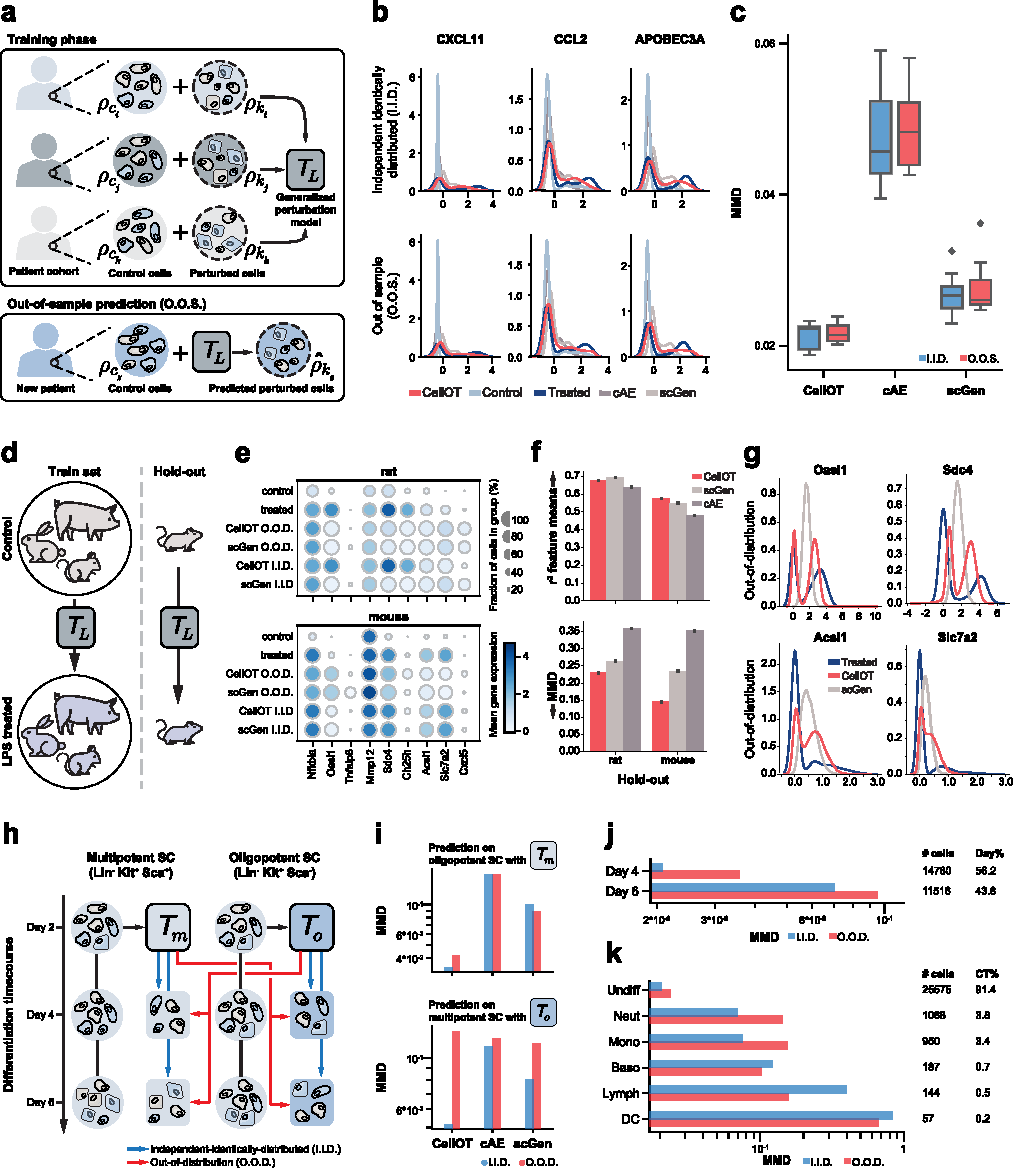
\includegraphics[width=0.6\textwidth]{figures/cellot-methods/Bunne_Main_Fig4.pdf}
  \end{center}
  \caption{
  \textsc{CellOT} generalizes to unseen patients and cell subpopulations.
  Out-of-sample (o.o.s., \textbf{a-c}), and out-of-distribution (o.o.d., \textbf{d-k}) setting.
  \textbf{a)} Predicting IFN-$\beta$ responses in distribution and out-of-sample. 
  \textbf{b)} Marginals of predicted cells from the holdout sample in the i.i.d.~(top) and o.o.s.~(bottom) setting. 
  \textbf{c)} MMD scores between the predicted distribution and the observed treated distribution across all holdout samples in the i.i.d.~and o.o.s.~settings.
  \textbf{d)} \textsc{CellOT} and baselines predict LPS response across heldout rat and mouse species
  \textbf{e)} Mean gene expression for i.i.d. and o.o.d. predictions for \textsc{CellOT} and \textsc{scGen} for selected marker genes.
  \textbf{f)} Comparison of o.o.d. performance for $r^2$ correlation feature means and MMD of \textsc{CellOT} and baselines. Data is depicted as the mean +/- standard deviation across n=10 bootstraps of the test set.
  \textbf{g)} Marginals of the o.o.d. predictions for marker genes showing bimodal expression profiles when using rat as a holdout.
    \textbf{h)} Cells from multipotent and oligopotent subpopulations develop for 6 days. \textsc{CellOT} predicts how cells from day 2 develop into the combined set of day 4 and 6, training on a single subpopulation.
    \textbf{i)} MMD scores between the predicted and (observed) developed distributions for all models in both o.o.d.~ and i.i.d.~prediction tasks (jointly for day 4 and 6). Performance of \textsc{CellOT}, when predicting \textbf{j)} day 4 states and day 6 states \textbf{k)} for different cell types in each setting using $T_m$.}
  \label{fig:cellot-main-ood}
\end{figure}


The maps between molecular states before and after treatments learned by \textsc{CellOT} contribute to a better understanding of the differences between cells that respond to certain drugs and cells that do not respond. This is crucial for inferring an incoming patient's response to drugs and settings with high cell-to-cell variability.
To make predictions on unseen patients, however, we need to demonstrate that the learned maps $T$ model perturbation responses across different patients coherently and robustly, while still predicting personalized treatment outcomes for each patient instead of mere population averages.
To test the generalization capacity of \textsc{CellOT} in such an out-of-sample scenario, we use a peripheral blood mononuclear cells (PBMC) droplet scRNA-seq dataset. \citet{kang2018} characterize the cell type specificity and inter-individual variability of the response of eight lupus patients to interferon beta (IFN-$\beta$), a potent cytokine that induces genome-scale changes in immune cell transcriptional profiles.
In the following, we compare the performance of \textsc{CellOT} and other baselines in an independent-and-identically-distributed (i.i.d.) setting, where models see cells from all patients, as well as in the out-of-sample (o.o.s.) setting, where models do not see cells from a specific holdout patient (see figure \ref{fig:cellot-main-ood}a).

As in the previous analysis, we evaluate how accurately \textsc{CellOT} captures the change in the overall expression of different marker genes from control to IFN-$\beta$-treated cells and thus how well the predicted gene expression marginals are aligned with the treated population (figure \ref{fig:cellot-main-ood}b). Here, we consider the genes \textit{CXCL11}, \textit{CCL2}, and \textit{APOBEC3A},
since they are connected with autoimmune diseases, including systemic lupus erythematosus \cite{hedrich2011, perez-bercoff2021}
and thus potential therapeutic targets
in the management of patients with lupus and, likely, other interferonopathies \cite{mathian2015,rani1996,hedrich2011,mathian2015,perez-bercoff2021,flier2001}.
% CXCL11 and CCL2 are both chemokines
% induced by IFN-$\beta$ \cite{need} and have been shown to play a very prominent and often interchangeable role in the mobilization of T cells during a variety of pathological conditions, including cancer, infection, and inflammation, making them potential therapeutic targets \cite{need}.
% Similarly, the cytidine deaminase APOBEC3 contributes epigenetically to autoimmune diseases such as systemic lupus erythematosus \cite{need} and is a potential subject in therapies targeting interferons and specifically A3 enzymes in the management of patients with lupus and probably other interferonopathies \cite{need}.
These selected genes show a large change in expression from the control to the perturbed population, partially exhibiting a bimodal gene expression profile upon perturbation. In contrast to \textsc{CellOT}, the baselines do not accurately predict these large transcriptomic shifts of these genes.
An extended analysis of additional genes strongly affected by the IFN-$\beta$ treatment can be found in Supplemental Figures \ref{supp_fig:lupus_all_marginals_iid} and \ref{supp_fig:lupus_all_marginals_ood}.

All models, including \textsc{CellOT}, show little performance drop when modeling the treatment outcome on a new patient using the generalized perturbation model $T_L$ trained on the patient cohort and using the control cells $\mu_z$ of the unseen patient as input.
This becomes evident when comparing the predicted population $\hat{\nu}_z$ with observations $\nu_z$ using the MMD metric. figure \ref{fig:cellot-main-ood}c displays summary results in which each individual patient was considered for the holdout set.
Further evaluation metrics, including the $\ell_2(\text{DS})$ score, can be found in Supplemental Figure \ref{supp_fig:lupus_iid_ood_l2ds}.
\textsc{CellOT} outperforms previous baselines both in the i.i.d.~and in the o.o.s.~setting, while further showing a smaller performance drop when generalizing to the unseen patient.
For more results, see Supplemental Figure \ref{supp_fig:lupus_umaps_all}.
These results suggest that the learned optimal transport maps correctly model the shift in the structures of the cellular subpopulation present in all patients, thus robustly performing out-of-sample.
We repeat the same evaluation for a glioblastoma cohort consisting of seven patients \cite{zhao2021}.
However, generalization within this setting proved to be difficult for \textsc{CellOT} and all baselines, due to the small size of the cohort and high degree of variance within the responses of each individual. 
% We have identified under which conditions generalization to unseen patients is feasible. 
For a complete analysis, see Supplemental Figure \ref{supp_fig:gbm_patients_iid_ood}.

\subsection{CellOT reconstructs innate immune responses across species}

The innate immune response is a cell-intrinsic defense program showing high levels of heterogeneity among responding cells -- and thus an ideal task for evaluating \textsc{CellOT}'s capabilities.
We rely our analysis on the dataset collected by \citet{hagai2018}, which studies the evolution of innate immunity programs of mononuclear phagocytes within different species, including pigs, rabbits, mice, and rats.
For this, these primary bone marrow-derived cells are stimulated using lipopolysaccharide (LPS).
In the following, we test how well \textsc{CellOT} and the baselines reconstruct innate immune responses within species that are not encountered during training.
We refer to the generalization task as out-of-distribution (o.o.d.), since unlike the o.o.s.~setting, we expect different species to have very distinct responses (see figure \ref{fig:cellot-main-ood}d).
The holdout set thereby consists of cells derived from either rat or mouse. See Supplemental Figure \ref{supp_fig:crossspecies_ood_analysis}a,b for an analysis of cross-species similarity and the reasoning behind selecting the holdout set.

Indeed, \textsc{CellOT} accurately reconstructs the innate immune response in both mouse and rat in the i.i.d. and o.o.d. setting.
This not only becomes evident through capturing more precisely the mean expression level of marker genes that show high differential expression levels upon addition of LPS, e.g., \textsc{Nfkb1} (NF-$\kappa$B), \textsc{Oasl1} (Oasl1), \textsc{Mmp12}, and \textsc{Cxcl5} (see figure \ref{fig:cellot-main-ood}e and Supplemental Figure \ref{supp_fig:crossspecies_ood_analysis}c-d), but also through the average correlation coefficient $r^2$ computed between o.o.d. predictions and holdout observations across all genes (see figure \ref{fig:cellot-main-ood}f).
In particular, \textsc{CellOT} outperforms the baselines when analyzing how well each method captures the heterogeneity of innate immune responses in different species, as demonstrated by low levels of MMD (see figure \ref{fig:cellot-main-ood}f).
Most impressively, our method shows a strong alignment or gene expression marginals of aforementioned marker genes that show complicated bimodal expression profiles upon perturbation (see figure \ref{fig:cellot-main-ood}g).

% \subsection*{CellOT generalizes perturbation responses out-of-distribution from multipotent populations to cells of lower potency}
\subsection{CellOT extends differentiation results to cells of lower potency}

During developmental processes, stem and progenitor cells progress through a hierarchy of fate decisions, marked by a continuous differentiation of cells that refine their identity until reaching a functional end state.
% Modern high-throughput methods allow us to monitor these successive changes in gene expression profiles by observing multiple snapshots over time. To ultimately associate molecular differences among progenitor cells with their capacity to generate mature cell types and get a better understanding of biological differentiation or reprogramming mechanisms, we are required to learn the alignment of progenitor to mature cell states.
By tracking an initial cell population along the differentiation process, \textsc{CellOT} allows us to recover individual molecular cell fate decisions and developmental trajectories. 
% Here, the perturbation of the control population of progenitor cells is initiated by internal molecular factors driving developmental processes instead of some external factor. 
% \citet{weinreb2020lineage} use the mouse hematopoietic system as a model for a developmental process. To be able to clonally trace transcriptomes over time and capture not only each transcriptional cell state but also fate, each cell contains a genetic barcode that remains throughout cell division. This not only allows one to detect sister cells in the earliest stages of the developmental process but also links differentiated cells sampled at a later stage of the differentiation process to the original cell by reading out the barcode.

\citet{weinreb2020} analyzed the fate potential of hematopoietic stem and progenitor cells (HSPCs), by tracking a broad class of oligopotent %(LIN$^{-}$KIT$^{+}$SCA$^{-}$) 
and multipotent %(LIN$^{-}$KIT$^{+}$SCA$^{+}$)
progenitor cell subpopulations and observing samples on days 2, 4, and 6 (Figure \ref{fig:cellot-main-ood}h).
Here, we test how well \textsc{CellOT} and other baselines can learn the differentiation process of the cells observed on day 2 to the cells observed on days 4 and 6 (combined) and generalize from one subpopulation to another (o.o.d. setting).
% Similar to the o.o.s. setting, we train two models per each subpopulation.
We learn two maps, where map $T_o$ is trained exclusively on oligopotent cells, $T_m$ on multipotent cells.
I.i.d.~versions of these maps are trained on both oligopotent and multipotent cells, such that each pair of i.i.d.~and o.o.d.~maps is evaluated on the same test set.
Comparing the distributional distance between predicted and observed differentiated cell states using the MMD metric, \textsc{CellOT} outperforms current state-of-the-art methods in this i.i.d.~setting for both the oligopotent and the multipotent subsets (see Figure \ref{fig:cellot-main-ood}i).
Furthermore, while baselines struggle to perform in either o.o.d.~setting, \textsc{CellOT} is able to generalize its predictions in one direction, i.e., from multipotent cells to the oligopotent setting.
In contrast to oligopotent cells, multipotent cells have a higher potency and thus can potentially differentiate into more cell types, and so we would expect $T_m$ is more likely to generalize than $T_o$, trained on the less potent oligopotent cells.
When predicting developmental perturbations on multipotent cells using $T_o$, the differentiated cell fates cannot be recovered.

We further compare the performance at different time points and across cell types.
Figure \ref{fig:cellot-main-ood}j shows the accuracy of the modeled development of multipotent cells using map $T_m$ individually for day 4 and day 6 cells, respectively.
It is evident that \textsc{CellOT} achieves better results when predicting developmental dynamics short-range instead of states further away in time (further results in Supplemental Figure \ref{supp_fig:statefate_shared_umaps}).
This suggests a potential limitation for all of these methods, which might be unable to recover alignments over coarse time resolutions.
Beyond, while the vast majority of cells on days 4 and 6 are still undifferentiated (undiff), some cells have evolved into neutrophils (neut), monocytes (mono), basophils (baso), lymphoid precursors (lymph), or dendritic cells (DC).
As expected, the performance of \textsc{CellOT} drops in terms of the MMD metric for those cell types that are only sparsely represented in the dataset (see Fig.~\ref{fig:cellot-main-ood}k).
